% Asset ID: FA22ChiSquaredTestsTikZ-001
% Topic ID: FA22ChiSquaredTests
% Unit: FA22 Further A2 2 Applied Mathematics
% Topic code: FA22-CHI2
% Related lesson file: FA22_chi_squared_tests_lesson.md
% Source: CCEA FA22-CHI2 specification + chi-squared distribution evidence
% Purpose: Precise mathematical sketch of a chi-squared distribution with upper-tail critical region.
\documentclass[tikz,border=8pt]{standalone}
\usepackage{amsmath,xcolor}
\usetikzlibrary{arrows.meta}
\definecolor{Canvas}{HTML}{FAF9F6}\definecolor{Ivory}{HTML}{FFFFF0}\definecolor{Line}{HTML}{E5E5EA}\definecolor{Gold}{HTML}{C5A059}\definecolor{SoftPink}{HTML}{FBEFEF}\definecolor{Text}{HTML}{2C2C2E}
\begin{document}
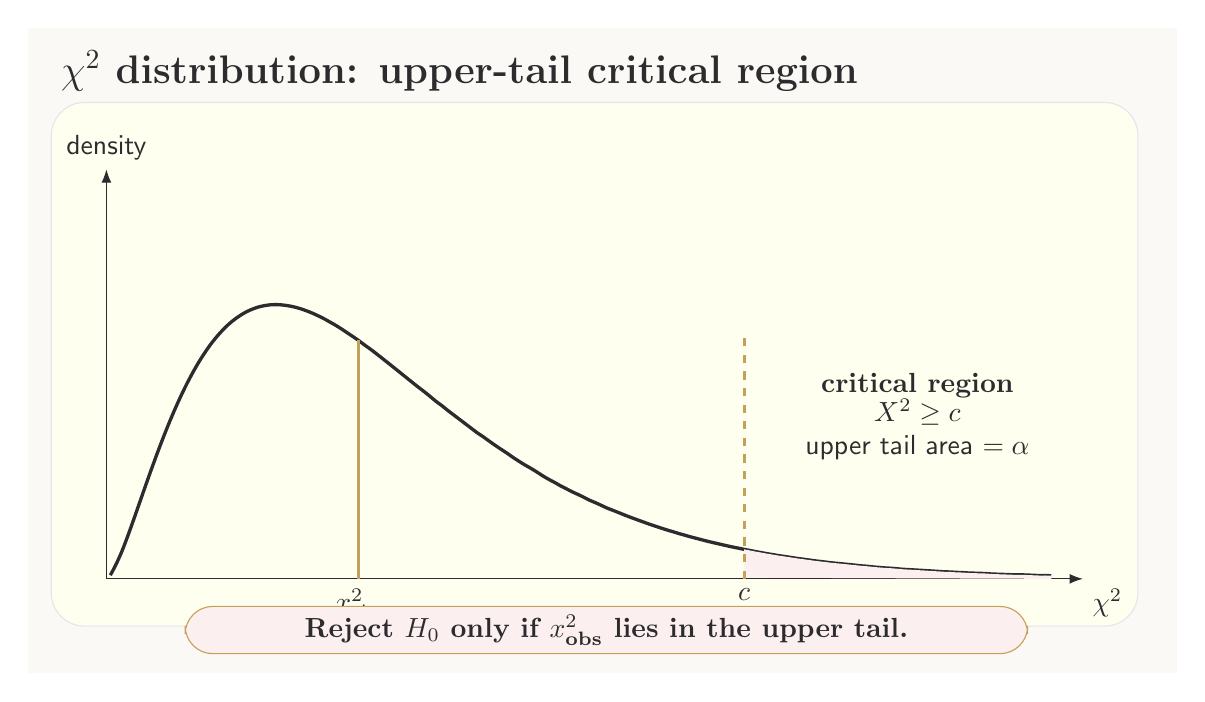
\begin{tikzpicture}[>=Latex,font=\sffamily,every node/.style={text=Text}]
\fill[Canvas] (-1,-1.2) rectangle (13.6,7);
\node[anchor=west,font=\bfseries\Large] at (-0.7,6.45){\(\chi^2\) distribution: upper-tail critical region};
\filldraw[fill=Ivory,draw=Line,rounded corners=12pt] (-0.7,-0.6) rectangle (13.1,6.05);
\draw[Text,->] (0,0)--(12.4,0) node[below right]{\(\chi^2\)};
\draw[Text,->] (0,0)--(0,5.2) node[above]{density};
\draw[Text,line width=1.2pt,smooth,domain=0.05:12,samples=160] plot (\x,{5.0*(\x)^1.55*exp(-0.72*\x)});
\def\crit{8.1}\def\xobs{3.2}
\begin{scope}\clip (\crit,0) rectangle (12.4,5.2);\fill[SoftPink] plot[smooth,domain=0.05:12,samples=160] (\x,{5.0*(\x)^1.55*exp(-0.72*\x)}) -- (12,0)--cycle;\end{scope}
\draw[Gold,dashed,line width=1.1pt] (\crit,0)--(\crit,3.1);\node[below] at (\crit,0){\(c\)};
\draw[Gold,line width=1pt] (\xobs,0)--(\xobs,{5.0*(\xobs)^1.55*exp(-0.72*\xobs)});\node[below] at (\xobs,0){\(x_{\text{obs}}^2\)};
\node[align=center,font=\bfseries] at (10.3,2.45){critical region};\node[align=center] at (10.3,1.9){\(X^2\ge c\)\\upper tail area \(=\alpha\)};
\filldraw[fill=SoftPink,draw=Gold,rounded corners=10pt] (1,-0.95) rectangle (11.7,-0.35);\node[font=\bfseries] at (6.35,-0.65){Reject \(H_0\) only if \(x_{\text{obs}}^2\) lies in the upper tail.};
\end{tikzpicture}
\end{document}
